\documentclass[fleqn,10pt,serif,xcolor=svgnames,xcolor=table,aspectratio=169,handout]{beamer}
% \includeonlyframes{current}
%========================================
% Packages
%========================================

\usepackage[palatino]{../../99-auxiliary-files/00-mypackBeamer}
\usepackage{../../99-auxiliary-files/00-mycommands}
\usepackage{../../99-auxiliary-files/00-myenvironments-beamer}

\usepackage{tikz-qtree}
\usepackage{array}
\usepackage[absolute,overlay]{textpos}
\usepackage{ulem}

%========================================
% More Layout (Beamer Special)
%========================================

\DefineNamedColor{named}{mycol}{cmyk}{0.6,0.6,0,0}
% \DefineNamedColor{named}{mygray}{cmyk}{0.05,0.05,0.05,0.05}
% \DefineNamedColor{named}{mygraylight}{cmyk}{0.017,0.017,0.017,0.017}

\definecolor{signal1}{rgb}{0.69, 0.25, 0.21}
\definecolor{signal2}{rgb}{1.0, 0.66, 0.07}
\definecolor{signal3}{rgb}{0.39, 0.58, 0.93}
\definecolor{signal4}{rgb}{0.0, 0.4, 0.0}
\definecolor{firebrick}{rgb}{0.7, 0.13, 0.13}
\definecolor{themecolor}{rgb}{0.3, 0.36, 0.33} % feldgrau
\definecolor{darkgray}{rgb}{0.66, 0.66, 0.66}

% \usetheme[height=7mm]{Rochester}
%\usetheme{Warsaw}


\usecolortheme{dove}

% \useoutertheme[compress,subsection=false]{miniframes}

\usecolortheme[named=themecolor]{structure}

\setbeamercolor{title}{fg=themecolor}

% \setbeamercolor{lower separation line head}{bg=white}

%\setbeamercolor{structure}{fg=Brown}
%\setbeamercolor{normal text}{fg=Brown}
%\setbeamercolor{section in head/foot}{bg=gray!40}
%%\setbeamercolor{lower separation line head}{bg=black!40}
%\setbeamercolor*{frametitle}{fg=Black,bg=gray!40}
%\setbeamercolor*{block body}{fg=Brown,bg=gray!00}
%\setbeamercolor*{block title}{fg=Black,bg=gray!40}


% Switch of shadows of boxes
\setbeamertemplate{blocks}[default]

% Frame numbers in footer
\setbeamertemplate{footline}[frame number]

% See-through preview for uncovered
% \setbeamercovered{transparent}

% Switch off navigation panel at bottom right
\beamertemplatenavigationsymbolsempty

% Change Style for itemize markers
% Options are ball, circle, rectangle and default (=triangle)
\setbeamertemplate{items}[circle]



\setcounter{tocdepth}{1}

% Use bullets in enumerates and TOC
\setbeamertemplate{enumerate item}[circle]

% Set color for enumerate/TOC bullets to white
\setbeamercolor*{item projected}{fg=themecolor,bg=gray!00}

\setbeamercolor*{author}{fg=gray!80}

\setbeamerfont*{block title}{size=\normalsize}
\setbeamerfont*{title}{size=\huge}
\setbeamerfont*{subtitle}{size=\large}

% \newcommand{\mygray}[1]{{\color{gray}{#1}}}
% \newcommand{\mycol}[1]{{\color{mycol}{#1}}}

\newcommand{\mycomment}[1]{\hfill {\mygray{#1}}}
\newcommand{\mycom}[1]{\hfill {\mygray{[#1]}}}

\newcommand{\slideFN}[1]{%
  \begin{textblock*}{\paperwidth}(0pt,1.05\textheight)
    \hfill \footnotesize{\mygray{#1}} \hspace{.5em}
  \end{textblock*}}

\newcommand{\pictureslide}[2][current]{
\usebackgroundtemplate{\includegraphics[width=\paperwidth]{#2}}%
\begin{frame}[label=#1]

\end{frame}
}
% code below makes it possible to turn inclusion of frames
% into 'miniframes' off and on with commands:
% \miniframeson and \miniframesoff
% from: http://tex.stackexchange.com/questions/37127/how-to-remove-some-pages-from-the-navigation-bullets-in-beamer

\makeatletter
\let\beamer@writeslidentry@miniframeson=\beamer@writeslidentry
\def\beamer@writeslidentry@miniframesoff{%
  \expandafter\beamer@ifempty\expandafter{\beamer@framestartpage}{}% does not happen normally
  {%else
    % removed \addtocontents commands
    \clearpage\beamer@notesactions%
  }
}
\newcommand*{\miniframeson}{\let\beamer@writeslidentry=\beamer@writeslidentry@miniframeson}
\newcommand*{\miniframesoff}{\let\beamer@writeslidentry=\beamer@writeslidentry@miniframesoff}
\makeatother

\setbeamertemplate{bibliography item}{}


%========================================
% Commands
%========================================

\newcommand{\mycol}[1]{{\textcolor{mycol}{#1}}}
\renewcommand{\markdef}[1]{\mycol{#1}}
\newcommand{\mygray}[1]{\textcolor{gray}{#1}}
\definecolor{darkgray}{rgb}{0.66, 0.66, 0.66}

\renewcommand{\slideFN}[1]{%
  \begin{textblock*}{\paperwidth}(0pt,0.95\textheight)
    \hfill \footnotesize{\mygray{#1}} \hspace{.5em}
  \end{textblock*}}

\newcommand{\proplog}{\acro{PropLog}}
\newcommand{\predlog}{\acro{PredLog}}

\renewcommand{\mymark}[1]{\textbf{{\textcolor{themecolor}{ #1}}}}

\def\checkmark{\tikz\fill[scale=0.4](0,.35) -- (.25,0) -- (1,.7) -- (.25,.15) -- cycle;}

%========================================
% Document
%========================================

\title{Predicate logic: semantics}
\subtitle{Methods: Logic, Part 5}

\author{Michael Franke}
\date{}


%--------------------------------------

\begin{document}

% --- Horizontal Space Fix ----

\abovedisplayskip=3pt
\abovedisplayshortskip=3pt

\belowdisplayskip=3pt
\belowdisplayshortskip=3pt

\begin{frame}
  \maketitle
\end{frame}

\begin{frame}

  \begin{minipage}{0.45\linewidth}
    \centering
    \mymark{Propositional logic} \\ \medskip
    $V(\varphi) \in \set{0,1}$
  \end{minipage}
  \hfill
  \begin{minipage}{0.45\linewidth}
    \centering
    \mymark{Predicate logic} \\ \medskip
    $V_{\textcolor{signal1}{M}}(\varphi) \in \set{0,1}$
  \end{minipage}

\end{frame}


\begin{frame}
  \frametitle{Model of predicate logic}


  A model $M = \tuple{D, I}$ for $\mathfrak{L}$ consists of:
    \begin{itemize}
    \item[] domain $D \neq \emptyset$: set of entities
      \item[] interpretation function $I$:
      \begin{itemize}
        \item[] if $c$ is a constant of $\mathfrak{L}$, then $I(c) \in D$, and
        \item[] if $P$ is an $n$-ary predicate letter of $\mathfrak{L}$, then $I(P) \subseteq D^n$.
      \end{itemize}
    \end{itemize}


  \slideFN{$D^n$ is the set of all $n$-tuples with elements from $D$}

\end{frame}

\begin{frame}
  \frametitle{Assignments and term interpretations}

  \begin{block}{Assignment function}
    An \mymark{assignment function} $g$ for model $M = \tuple{D,I}$ and language $\mathfrak{L}$ maps all
    variables in $\mathfrak{L}$ to elements in $D$.
  \end{block}

  \begin{block}{Term interpretation}
    If $t$ is a term of $L$, then $\den{t}_{M,g}$ is the \mymark{term interpretation} relative to $M = \tuple{D,I}$ and $g$:
    \begin{multicols}{2}
      \begin{itemize}
      \item[] $\den{t}_{M,g} = I(t)$ if $t$ is a constant, and
      \item[] $\den{t}_{M,g} = g(t)$ otherwise.
      \end{itemize}
    \end{multicols}

  \end{block}

\end{frame}

\begin{frame}
  \frametitle{Valuation functions for predicate logic (1)}

  \begin{block}{Simple formulas}
    \begin{tabular}{lcl}
      $V_{M,g}(At_1\dots t_n) =1$ & iff & $\tuple{\den{t_1}_{M,g}, \dots, \den{t_n}_{M,g}} \in I(A)$
    \end{tabular}
  \end{block}

\begin{block}{Sentential connectives}
    \begin{tabular}{lcl}
      $V_{M,g}(\neg \phi) = 1$ & iff & $V_{M,g}(\phi) =0$\\
      $V_{M,g}(\phi \wedge \psi) = 1$ & iff & $V_{M,g}(\phi) =1$ and $V_{M,g}(\psi) = 1$\\
      $V_{M,g}(\phi \vee \psi) = 1$ & iff & $V_{M,g}(\phi) =1$ or $V_{M,g}(\psi) = 1$\\
      $V_{M,g}(\phi \rightarrow \psi) = 0$ & iff & $V_{M,g}(\phi) =1$ and $V_{M,g}(\psi) = 0$\\
      $V_{M,g}(\phi \leftrightarrow \psi) = 1$ & iff & $V_{M,g}(\phi) = V_{M,g}(\psi)$
    \end{tabular}
  \end{block}

\end{frame}


\begin{frame}
  \frametitle{Valuation functions for predicate logic (2)}

  \begin{block}{Quantifiers}
    \begin{tabular}{lcl}
      $V_{M,g}(\forall x \myts \phi) = 1$ & iff & $V_{M,g_{[x/d]}}(\phi) = 1$ for all $d \in D$\\
      $V_{M,g}(\exists x \myts \phi) = 1$ & iff & $V_{M,g_{[x/d]}}(\phi) = 1$ for at least one $d \in D$
    \end{tabular}
  \end{block}


  \begin{block}{Notation}
    We write $g_{[x/d]}$ and read ``$g$ with $x$ mapped to $d$,'' for the assignment function
    which is like $g$ except that $x$ is mapped to $d \in D$.
  \end{block}

\end{frame}


\begin{frame}
  \frametitle{Truth in a model}

    If $V_{M,g}(\phi) = 1$ for all $g$, we write $V_{M}(\phi) = 1$ and say ``$\phi$ is true in
    $M$''. \\
    Similarly for \textit{false}. \\
    Any sentence (no free variables) is either true or false in any given model $M$.

\end{frame}

\begin{frame}
  \frametitle{Example}

  \begin{block}{Model}
  \begin{minipage}{0.45\linewidth}
    \centering
    \begin{align*}
      D    & = \set{1,2,3,4,5}\\
      I(a) & = 3 \\
      I(P) & = \set{1,2,5} \\
      I(Q) & = \set{2,5} \\
      I(R) & = \set{\tuple{1,2},\tuple{2,2}, \tuple{1,4}, \tuple{1,5}}
    \end{align*}
  \end{minipage}
  \hfill
  \begin{minipage}{0.45\linewidth}
    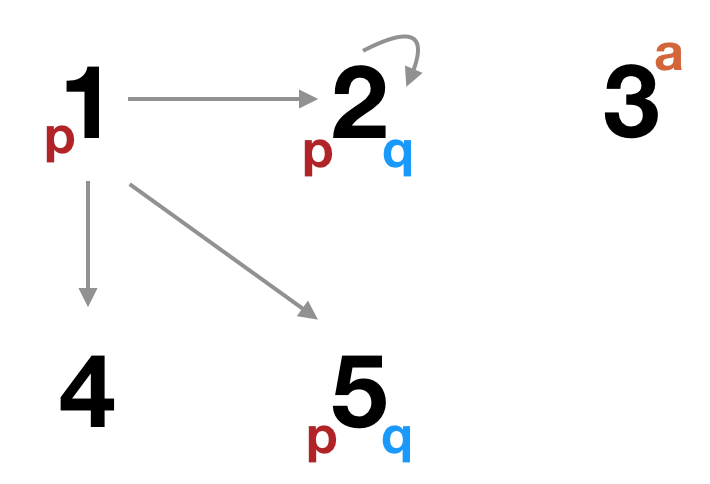
\includegraphics[width=0.8\textwidth]{../../01-handouts/00-pics/predlog-example-model.png}
  \end{minipage}
\end{block}

  \bigskip \pause

  \hrule

  \bigskip

  \begin{block}{Truth of formulas in the model}
  \begin{multicols}{2}
    \begin{enumerate}[(i)]
      \item $V_{M}(\exists x \myts (Px \wedge Qx) ) = 1$
      \item $V_{M}(Pa) = 0$
      \item $V_{M}(\forall x \myts (Px \rightarrow Qx)) = 0$
      \item $V_{M}(\forall x \myts (Rax \rightarrow Qx)) = 1$
  \end{enumerate}
  \end{multicols}
\end{block}


\end{frame}

% \begin{frame}
%   \frametitle{Validity}

%   \begin{block}{Argument schema}
%     If $\phi_1, \dots, \phi_n$ and $\psi$ are sentences of predicate logic, $\phi_1, \dots,
%     \phi_n / \psi$ is an \mymark{argument schema}.
%   \end{block}

%   \begin{block}{Validity}
%     The argument schema $\phi_1, \phi_2, \dots, \phi_n / \psi$ is \markdef{valid} iff for all
%     models $M$ such that $V_M(\phi_1)=V_M(\phi_2)= \dots = V_M(\phi_n)=1$ it also holds
%     that $V_M(\psi) = 1$. \\
%     If valid, we write $\phi_1, \phi_2, \dots, \phi_n \models \psi$.
%   \end{block}

% \end{frame}

% \begin{frame}
%   \frametitle{Counterexamples to validity}

%   Show that the argument schemas below are not valid by giving a counterexample.

%   \begin{enumerate}[(a)]
%   \item $\exists x \, Ax, \ \exists x \, Bx \ / \ \exists x \, (Ax \wedge Bx)$
%   \item $\forall x \, (Ax \vee Bx) \ / \ \forall x \, Ax \vee \forall x \, Bx$
%   \item $\forall x \, (Ax \rightarrow Bx) \ , \ \exists x \, Bx \ / \ \neg \exists x \, Ax$
%   \end{enumerate}

% \end{frame}


\end{document}
